\section{Theory}
The purpose of this chapter is to explain the most important terms about blockchain and the key underlying components of the technology.
Most explanations will be kept superficial, as only a broad understanding of the term is required for this thesis.
\\\\

\textbf{Cryptocurrency}\\
Traditional, so-called fiat currencies like the Euro or US Dollar, have been around for hundreds of years in form of coins or paper money.
They are usually issued and regulated by a government.
With the internet a new form of currencies, the so-called cryptocurrencies emerged.
They are digital currencies that are usually decentralized, meaning they work without a central authority controlling and regulating the flow of monetary value.
The rightfulness of transactions is ensured by mathematical functions like digital signatures and often a technology called the blockchain.
\\\\

\textbf{Hash}\\
In cryptocurrencies, hashes are used to verify data.
The cryptographic hash function is a mathematical function that usually fulfills the following requirements\cite{hash}:
\begin{enumerate}
    \item \textit{Determinism}: the same input always produces the same output
    \item \textit{Preimage resistance}: it's nearly impossible to get the input from the output
    \item \textit{Second-preimage resistance}: it's nearly impossible to find a second input that produces the same output as the first input
\end{enumerate}
The output of this function is called hash.
Bitcoin uses the SHA-256\cite{bitcoin-whitepaper}, Ethereum uses the Keccak-256\cite{ethereum-yellow-paper} hashing algorithm which produces an output hash with a length of 32 bytes.
\\\\

\textbf{Public Key Cryptography}\\
Public key cryptography\cite{public-key-cryptography} is the backbone of the blockchain technology and consists of a key pair – a private and a public key.
As the name suggests the private key needs to be secret and the public key can be shared with anyone.
A message can be signed using the private key resulting in a signature.
This signature can then be verified using the public key to prove that the message was, in fact, signed by the corresponding private key.
Bitcoin and Ethereum use the \abbr{Elliptic Curve Digital Signature Algorithm}{ECDSA} for signatures.
They are used to prove that transactions were indeed sent by a specific account and not manipulated.
\newpage

\textbf{Wallet}\\
Everything that is needed to send and/or receive cryptocurrencies is a private key\cite{bitcoin-whitepaper}, which is a wallet in its simplest form.
More complex forms of a wallet encrypt a private private key with a password or store it on a dedicated hardware device.
\\\\

\textbf{Address}\\
An address is used to identify participants on the blockchain.
Usually it's derived from a public key belonging to the private key of an account, e.g. Ethereum uses the 20 least significant bytes of the Keccak-256 hash of the public key as the address\cite{ethereum-yellow-paper}.
\\\\

\textbf{Ledger}\\
The ledger is the equivalent of a traditional record of all addresses and their balances.
Every participant of the network has a copy of this ledger.
\\\\

\textbf{Node}\\
A node is a participant on the blockchain.
When a new node joins the network, it downloads the ledger, currently accepted by the majority.
A so-called full node has the entire history of the ledger – from the first block to the latest.
\\\\

\textbf{Transaction}\\
A transaction updates the ledger, e.g. reducing the balance of an address by a specific amount and adding it to the balance of another account.
\\\\

\textbf{Blockchain}\\
A list of transactions is bundled together into a block.
Also included in this block is the hash of the previous block, which contains the hash of the previous block and so on.
This creates a chain of blocks\cite{bitcoin-whitepaper} which always point to their predecessor as demonstrated in figure \ref{fig:blockchain}, thus the name blockchain.
This is also the reason why a blockchain is considered immutable: modifying any information in a block would automatically change the hashes of every block after it and would be rejected by the network.
\newpage
\begin{figure}[H]
    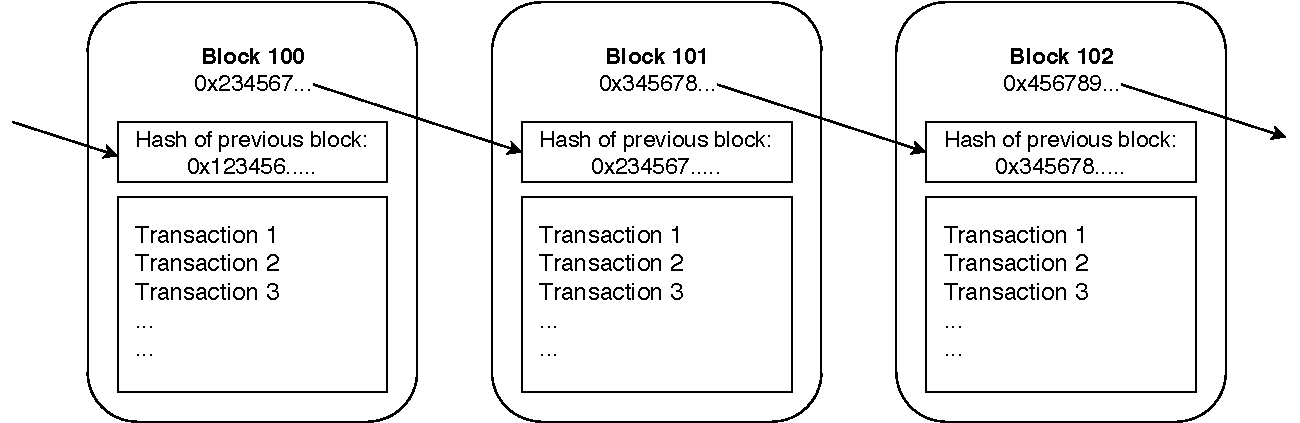
\includegraphics[width=\textwidth]{img/blockchain.pdf}
    \caption{Visualization of a blockchain}
    \label{fig:blockchain}
\end{figure}
\leavevmode
\\

\textbf{Miner / Validator}\\
A miner is a participant on the network whose task it is to secure the network through validating or mining new transactions and blocks.
\\\\

\textbf{Fees}\\
For most cryptocurrencies a fee has to be paid with every transaction.
These go to the miner as a reward for including a transaction in a block.
Additionally they prevent an attacker from spamming the network with transactions.
In contrast to traditional payment methods, which usually have a variable fee based on the total transaction value, cryptocurrencies have a fixed fee.
Miners can freely choose which transactions they want to include in a block, therefore the more a user is willing to pay, the higher the chance, that the transaction will be included in the next block.
Fees differ from cryptocurrency to cryptocurrency and can be as low as a fraction of a cent, but also went up to 55\$ for a single transaction on average\cite{btc-fees} for Bitcoin once, when the network couldn't scale to handle all transactions.
\\\\

\textbf{Proof of Work}\\
There are different approaches to reach consensus over which block should be added next to the network, \abbr{Proof of Work}{PoW} is one of them and is used by most cryptocurrencies.
A \abbr{number used once}{nonce} is included in the block which is adjusted by a validator.
Every different nonce produces a different block hash.
The goal is to find a nonce that is numerically lower than a certain threshold value (also called difficulty).
A validator who finds this number can submit their block to the network.
All miners race to find a nonce as fast as possible, so their block will be accepted by all other participants in the network and considered valid.
The fastest submission gets a so-called block reward, a reward minted by the protocol to the fastest miner, as well as all transaction fees from that block.
\newpage

\textbf{Block Time}\\
The time it takes to add a new block to the network is called block time.
On the Bitcoin network the block time is 10 minutes\cite{bitcoin-whitepaper}.
Ethereum wants to archive a block time of 12 seconds\cite{ethereum-blocktime}, realistically it's averaging at about 15 seconds\cite{ethereum-blocktime-chart}.
The difficulty is adjusted automatically to keep the block time roughly the same, no matter how much computing power is currently mining.
\\\\

\textbf{Confirmation Time}\\
The confirmation time is the time it takes until a transaction is mined.
The higher the transaction fee the faster the transaction is confirmed.
\\\\

\textbf{Ethereum Virtual Machine}\\
The \abbr{Ethereum Virtual Machine}{EVM} is a Turing complete virtual machine that can execute computer code on the Ethereum blockchain.
As a result, the Ethereum network acts like a decentralized computer with all the features of a blockchain: the storage is entirely public and every computation or code execution is recorded on the blockchain.
\\\\

\textbf{Smart Contract}\\
Smart contracts are written in special programming languages, the most popular being called "Solidity", and are compiled into bytecode afterwards.
This bytecode is then publicly stored on the blockchain and can be executed by everyone.
The advantage of smart contracts is, that the code is public to everyone and immutable, thus can theoretically be used as a binding, programmable contract that can control monetary value on its own.
As a drawback, every computational step and byte stored on the blockchain costs money in form of transaction fees.
\\\\

\textbf{DApp / Web3}\\
DApp stands for decentralized application.
Web3 is also called the decentralized web, where websites are powered by smart contracts and DApps.
\\\\

\textbf{Account}\\
There are two types of accounts on the Ethereum blockchain: An \abbr{externally owned account}{EOA} and a contract account.
Each of those accounts has a transaction count and a balance\cite{ethereum-yellow-paper} associated with them.
An EOA is controlled by a private key, whereas a contract account has code and storage associated with it.
\newpage

\textbf{Off-chain Transactions / Payment Channels}\\
For every transaction on the blockchain fees have to be paid.
One way to save transaction fees is to have multiple transactions that are not recorded on the blockchain.
They are called off-chain transactions and are settled on the blockchain, once the payment process is finished.
\\\\

\textbf{Ether - GWei - Wei}\\
\abbr{Ether}{ETH} is the currency used on the Ethereum network.
It can be divided into smaller fractions.
The most important are Wei and GWei.
Wei is the smallest unit: 1~Ether equals \(10^{18}\)~Wei\cite{ethereum-yellow-paper}.
GWei is primarily used for calculations of transaction fees: 1~Ether equals \(10^{9}\)~GWei, 1~GWei equals \(10^{9}\)~Wei.
Ether is always used in Wei format in smart contracts.
\\\\

\textbf{Mainnet / Testnet}\\
The main network of a blockchain is called the mainnet.
Testnets are blockchain networks that behave similarly to the official mainnet and are used for testing purposes only.
This allows developers to develop smart contracts without the risk of losing any monetary value.
Additionally, improvements to the mainnet are often tested on a testnet prior to their official implementation.